\documentclass[UTF8,zihao=-4]{ctexart}
\usepackage[a4paper,landscape,margin=0.8cm]{geometry}
\usepackage[table]{xcolor}
\usepackage{tikz}
\usetikzlibrary{arrows.meta,positioning}
\usepackage{array,tabularx}
\setlength{\parindent}{0pt}
\setlength{\parskip}{0.25em}
\pagestyle{empty}

\definecolor{bg}{HTML}{F7FAFC}
\definecolor{soft}{HTML}{EDF2F7}
\definecolor{b1}{HTML}{2B6CB0}
\definecolor{b2}{HTML}{DD6B20}
\definecolor{b3}{HTML}{2F855A}
\definecolor{b4}{HTML}{B83280}

\newcommand{\ptitle}[1]{\textbf{\Large #1}\par\vspace{0.12cm}\hrule\vspace{0.2cm}}
\newcommand{\source}{\footnotesize 数据来源：CCF《2025聚酯产业市场年度报告》（https://www.ccf.com.cn/newscenter/newsdetail-B00000-2025120600023.shtml）、品种框架报告模板、公开资料整理。}

\newcommand{\panel}[2]{%
\fcolorbox{black!25}{bg}{\begin{minipage}[t][4.6cm][t]{0.46\textwidth}
\textbf{#1}\par\vspace{0.1cm}
{\scriptsize #2}
\end{minipage}}}

\newcommand{\tinybars}{%
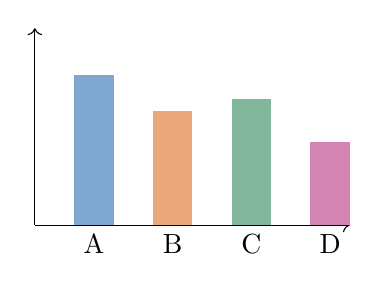
\begin{tikzpicture}[x=0.5cm,y=0.5cm]
\draw[->] (0,0)--(0,5);
\draw[->] (0,0)--(8,0);
\fill[b1!60] (1,0) rectangle (2,3.8);
\fill[b2!60] (3,0) rectangle (4,2.9);
\fill[b3!60] (5,0) rectangle (6,3.2);
\fill[b4!60] (7,0) rectangle (8,2.1);
\node[below] at (1.5,0) {A};\node[below] at (3.5,0) {B};\node[below] at (5.5,0) {C};\node[below] at (7.5,0) {D};
\end{tikzpicture}}

\newcommand{\tinyflow}{%
\begin{tikzpicture}[x=0.6cm,y=0.6cm]
\node[draw,rounded corners=1mm,fill=soft] (a) at (0,0) {成本};
\node[draw,rounded corners=1mm,fill=soft,right=1.2cm of a] (b) {开工};
\node[draw,rounded corners=1mm,fill=soft,right=1.2cm of b] (c) {库存};
\node[draw,rounded corners=1mm,fill=soft,right=1.2cm of c] (d) {价格};
\draw[-{Stealth[length=2mm]}] (a)--(b);
\draw[-{Stealth[length=2mm]}] (b)--(c);
\draw[-{Stealth[length=2mm]}] (c)--(d);
\end{tikzpicture}}

\begin{document}

% 1
\begin{center}
\vspace*{1.5cm}
{\Large w w w . c i e c . c o m\par}
\vspace{1.2cm}
{\fontsize{30}{36}\selectfont\bfseries 乙二醇框架报告（展示版）\par}
\vspace{0.5cm}
{\Large 汇报人：周文熙\par}
\vspace{0.3cm}
{\Large 2026.04\par}
\vfill
\end{center}
\newpage

% 2
\ptitle{目录与研究主线}
\begin{tabular}{p{0.48\textwidth} p{0.48\textwidth}}
\panel{目录}{一、产业结构\\二、全球供需格局\\三、国内供需格局\\四、价格价差\\五、交易标的} &
\panel{核心观点}{1) 乙二醇定价由成本、供给、库存、需求联动决定。\\2) 聚酯开工是需求侧最核心变量。\\3) 进口到港和港口库存决定短期波动。} \\
\panel{研究流程图}{\tinyflow} &
\panel{关键指标清单}{\begin{tabular}{|p{3.2cm}|p{6.4cm}|}\hline
指标&用途\\\hline
原料成本&判断成本中枢\\\hline
装置开工&判断供给弹性\\\hline
港口库存&判断现货压力\\\hline
聚酯负荷&判断需求强弱\\\hline
\end{tabular}}
\end{tabular}
\vfill\source
\newpage

% 3
\ptitle{一、产业结构：产业链总览}
\begin{tabular}{p{0.48\textwidth} p{0.48\textwidth}}
\panel{图3-1 产业链主图}{\begin{tikzpicture}[x=0.6cm,y=0.6cm]
\node[draw,fill=soft] (u) at (0,0) {上游原料};
\node[draw,fill=soft,right=1.6cm of u] (m) {生产工艺};
\node[draw,fill=soft,right=1.6cm of m] (e) {乙二醇};
\node[draw,fill=soft,below right=0.8cm and 0.6cm of e] (d) {聚酯下游};
\draw[-{Stealth[length=2mm]}] (u)--(m);
\draw[-{Stealth[length=2mm]}] (m)--(e);
\draw[-{Stealth[length=2mm]}] (e)--(d);
\end{tikzpicture}} &
\panel{图3-2 下游结构}{\tinybars}\\
\panel{图3-3 供需传导}{\tinyflow} &
\panel{表3-1 产业链环节}{\begin{tabular}{|p{2.7cm}|p{6.8cm}|}\hline
环节&说明\\\hline
上游&原油/煤/天然气\\\hline
中游&EO水合、煤制、合成气\\\hline
下游&长丝、短纤、瓶片\\\hline
\end{tabular}}
\end{tabular}
\vfill\source
\newpage

% 4
\ptitle{产业结构：工艺路线}
\begin{tabular}{p{0.48\textwidth} p{0.48\textwidth}}
\panel{图4-1 石脑油路线}{原油 $\rightarrow$ 石脑油 $\rightarrow$ 乙烯 $\rightarrow$ EO $\rightarrow$ EG\\\tinybars} &
\panel{图4-2 煤制路线}{煤炭 $\rightarrow$ 合成气 $\rightarrow$ 中间体 $\rightarrow$ EG\\\tinybars}\\
\panel{图4-3 气头路线}{天然气 $\rightarrow$ 合成气 $\rightarrow$ 中间体 $\rightarrow$ EG\\\tinybars} &
\panel{表4-1 工艺对比}{\begin{tabular}{|p{2.2cm}|p{2.2cm}|p{2.2cm}|p{1.8cm}|}\hline
路线&成本锚&优势&约束\\\hline
油头&油价&成熟&波动\\\hline
煤头&煤价&本地化&环保\\\hline
气头&气价&稳定&区域\\\hline
\end{tabular}}
\end{tabular}
\vfill\source
\newpage

% 5
\ptitle{产业结构：成本与利润}
\begin{tabular}{p{0.48\textwidth} p{0.48\textwidth}}
\panel{图5-1 成本曲线示意}{\tinybars} &
\panel{图5-2 利润弹性示意}{\tinybars}\\
\panel{图5-3 开停逻辑}{\tinyflow} &
\panel{表5-1 成本跟踪项}{\begin{tabular}{|p{3cm}|p{6.4cm}|}\hline
变量&含义\\\hline
原油/煤/气&成本中枢\\\hline
加工费&利润空间\\\hline
开工率&供给强弱\\\hline
\end{tabular}}
\end{tabular}
\vfill\source
\newpage

% 6
\ptitle{二、全球供需格局：供应结构}
\begin{tabular}{p{0.48\textwidth} p{0.48\textwidth}}
\panel{图6-1 全球供应区域}{\tinybars} &
\panel{图6-2 主要产区比较}{\tinybars}\\
\panel{图6-3 出口能力变化}{\tinybars} &
\panel{表6-1 区域特征}{\begin{tabular}{|p{2.8cm}|p{2.5cm}|p{3.8cm}|}\hline
区域&定位&影响\\\hline
中东&出口&边际供给\\\hline
北美&远洋&套利流向\\\hline
亚洲&消费&现货定价\\\hline
\end{tabular}}
\end{tabular}
\vfill\source
\newpage

% 7
\ptitle{全球供需格局：供应变化驱动}
\begin{tabular}{p{0.48\textwidth} p{0.48\textwidth}}
\panel{图7-1 能源价格影响}{\tinybars} &
\panel{图7-2 检修影响}{\tinybars}\\
\panel{图7-3 贸易影响}{\tinybars} &
\panel{表7-1 驱动拆解}{\begin{tabular}{|p{2.8cm}|p{6.2cm}|}\hline
驱动&说明\\\hline
原料&影响边际成本\\\hline
检修&影响短期产量\\\hline
运费&影响套利窗口\\\hline
\end{tabular}}
\end{tabular}
\vfill\source
\newpage

% 8
\ptitle{全球供需格局：需求结构}
\begin{tabular}{p{0.48\textwidth} p{0.48\textwidth}}
\panel{图8-1 需求去向}{\tinybars} &
\panel{图8-2 长丝需求}{\tinybars}\\
\panel{图8-3 瓶片需求}{\tinybars} &
\panel{表8-1 需求分层}{\begin{tabular}{|p{2.8cm}|p{6.1cm}|}\hline
层级&驱动\\\hline
长丝&纺服和出口\\\hline
短纤&替代和制造\\\hline
瓶片&包装和饮料\\\hline
\end{tabular}}
\end{tabular}
\vfill\source
\newpage

% 9
\ptitle{全球供需格局：物流流向}
\begin{tabular}{p{0.48\textwidth} p{0.48\textwidth}}
\panel{图9-1 中东至亚洲}{\tinyflow} &
\panel{图9-2 北美至亚洲}{\tinyflow}\\
\panel{图9-3 区域内部调货}{\tinyflow} &
\panel{表9-1 流向与价差}{\begin{tabular}{|p{3cm}|p{2.8cm}|p{2.8cm}|}\hline
流向&触发&含义\\\hline
中东-亚洲&套利开&进口增\\\hline
北美-亚洲&价差扩&远洋增\\\hline
亚洲内部&区域差&再分配\\\hline
\end{tabular}}
\end{tabular}
\vfill\source
\newpage

% 10
\ptitle{全球供需格局：平衡情景}
\begin{tabular}{p{0.48\textwidth} p{0.48\textwidth}}
\panel{图10-1 供给宽松情景}{\tinybars} &
\panel{图10-2 供给收缩情景}{\tinybars}\\
\panel{图10-3 需求改善情景}{\tinybars} &
\panel{表10-1 情景矩阵}{\begin{tabular}{|p{2.5cm}|p{2.5cm}|p{3.6cm}|}\hline
供给&需求&价格结果\\\hline
松&弱&偏弱\\\hline
松&强&震荡\\\hline
紧&强&偏强\\\hline
\end{tabular}}
\end{tabular}
\vfill\source
\newpage

% 11
\ptitle{全球供需格局：阶段小结}
\begin{tabular}{p{0.48\textwidth} p{0.48\textwidth}}
\panel{图11-1 全球框架复盘}{\tinyflow} &
\panel{图11-2 关键变量优先级}{\tinybars}\\
\panel{图11-3 领先与滞后指标}{\tinybars} &
\panel{表11-1 结论汇总}{\begin{tabular}{|p{3.0cm}|p{6.0cm}|}\hline
主题&结论\\\hline
供应&看边际出口\\\hline
需求&看聚酯负荷\\\hline
物流&看区域价差\\\hline
\end{tabular}}
\end{tabular}
\vfill\source
\newpage

% 12
\ptitle{三、国内供需格局：国产供给}
\begin{tabular}{p{0.48\textwidth} p{0.48\textwidth}}
\panel{图12-1 国产开工示意}{\tinybars} &
\panel{图12-2 检修节奏示意}{\tinybars}\\
\panel{图12-3 新产能节奏}{\tinybars} &
\panel{表12-1 国产供给观察点}{\begin{tabular}{|p{3.0cm}|p{5.8cm}|}\hline
指标&含义\\\hline
开工率&供给强弱\\\hline
检修&边际收缩\\\hline
投产&中期压力\\\hline
\end{tabular}}
\end{tabular}
\vfill\source
\newpage

% 13
\ptitle{国内供需格局：进口供给}
\begin{tabular}{p{0.48\textwidth} p{0.48\textwidth}}
\panel{图13-1 到港节奏}{\tinybars} &
\panel{图13-2 来源结构}{\tinybars}\\
\panel{图13-3 进口依赖变化}{\tinybars} &
\panel{表13-1 进口变量}{\begin{tabular}{|p{3.0cm}|p{5.8cm}|}\hline
变量&解释\\\hline
到港量&短期压力\\\hline
来源地&稳定性\\\hline
运费&套利效率\\\hline
\end{tabular}}
\end{tabular}
\vfill\source
\newpage

% 14
\ptitle{国内供需格局：需求结构}
\begin{tabular}{p{0.48\textwidth} p{0.48\textwidth}}
\panel{图14-1 长丝负荷}{\tinybars} &
\panel{图14-2 短纤负荷}{\tinybars}\\
\panel{图14-3 瓶片负荷}{\tinybars} &
\panel{表14-1 需求验证链}{\begin{tabular}{|p{2.8cm}|p{6.0cm}|}\hline
环节&验证方式\\\hline
订单&终端接单\\\hline
开工&聚酯负荷\\\hline
库存&去化速度\\\hline
\end{tabular}}
\end{tabular}
\vfill\source
\newpage

% 15
\ptitle{国内供需格局：库存中枢}
\begin{tabular}{p{0.48\textwidth} p{0.48\textwidth}}
\panel{图15-1 港口库存}{\tinybars} &
\panel{图15-2 厂内库存}{\tinybars}\\
\panel{图15-3 库存与现货}{\tinyflow} &
\panel{表15-1 库存信号}{\begin{tabular}{|p{2.8cm}|p{3.2cm}|p{2.6cm}|}\hline
状态&含义&价格\\\hline
累库&供给偏松&偏弱\\\hline
去库&需求偏强&偏强\\\hline
横盘&僵持&震荡\\\hline
\end{tabular}}
\end{tabular}
\vfill\source
\newpage

% 16
\ptitle{国内供需格局：区域物流}
\begin{tabular}{p{0.48\textwidth} p{0.48\textwidth}}
\panel{图16-1 港口至内地}{\tinyflow} &
\panel{图16-2 内地回流港口}{\tinyflow}\\
\panel{图16-3 区域价差与调货}{\tinybars} &
\panel{表16-1 物流观察}{\begin{tabular}{|p{3cm}|p{5.8cm}|}\hline
方向&含义\\\hline
港口-内地&现货消化\\\hline
内地-港口&库存回流\\\hline
跨区调货&价差驱动\\\hline
\end{tabular}}
\end{tabular}
\vfill\source
\newpage

% 17
\ptitle{国内供需格局：平衡场景}
\begin{tabular}{p{0.48\textwidth} p{0.48\textwidth}}
\panel{图17-1 高库存场景}{\tinybars} &
\panel{图17-2 去库存场景}{\tinybars}\\
\panel{图17-3 库存拐点场景}{\tinybars} &
\panel{表17-1 场景矩阵}{\begin{tabular}{|p{2.6cm}|p{2.6cm}|p{3.4cm}|}\hline
供给&需求&结果\\\hline
增&弱&累库\\\hline
减&强&去库\\\hline
稳&稳&横盘\\\hline
\end{tabular}}
\end{tabular}
\vfill\source
\newpage

% 18
\ptitle{国内供需格局：阶段小结}
\begin{tabular}{p{0.48\textwidth} p{0.48\textwidth}}
\panel{图18-1 国内框架复盘}{\tinyflow} &
\panel{图18-2 变量优先级}{\tinybars}\\
\panel{图18-3 信号验证顺序}{\tinybars} &
\panel{表18-1 核心结论}{\begin{tabular}{|p{2.8cm}|p{6cm}|}\hline
主题&结论\\\hline
供应&看开工+到港\\\hline
需求&看聚酯负荷\\\hline
库存&看港口变化\\\hline
\end{tabular}}
\end{tabular}
\vfill\source
\newpage

% 19
\ptitle{四、价格价差：价格驱动链}
\begin{tabular}{p{0.48\textwidth} p{0.48\textwidth}}
\panel{图19-1 成本到价格链}{\tinyflow} &
\panel{图19-2 供需到价格链}{\tinyflow}\\
\panel{图19-3 预期到盘面链}{\tinyflow} &
\panel{表19-1 驱动拆解}{\begin{tabular}{|p{2.8cm}|p{6cm}|}\hline
驱动&含义\\\hline
成本&价格下限\\\hline
库存&短期强弱\\\hline
预期&盘面弹性\\\hline
\end{tabular}}
\end{tabular}
\vfill\source
\newpage

% 20
\ptitle{价格价差：基差与月差}
\begin{tabular}{p{0.48\textwidth} p{0.48\textwidth}}
\panel{图20-1 基差框架}{\tinybars} &
\panel{图20-2 月差框架}{\tinybars}\\
\panel{图20-3 基差与库存}{\tinyflow} &
\panel{表20-1 结构解读}{\begin{tabular}{|p{2.8cm}|p{6cm}|}\hline
指标&解读\\\hline
基差&现货松紧\\\hline
月差&近远月预期\\\hline
联动&交易结构\\\hline
\end{tabular}}
\end{tabular}
\vfill\source
\newpage

% 21
\ptitle{价格价差：利润与跨品种价差}
\begin{tabular}{p{0.48\textwidth} p{0.48\textwidth}}
\panel{图21-1 乙二醇利润}{\tinybars} &
\panel{图21-2 EG-PTA关系}{\tinybars}\\
\panel{图21-3 EG-原料关系}{\tinybars} &
\panel{表21-1 价差观察}{\begin{tabular}{|p{2.8cm}|p{6cm}|}\hline
价差&用途\\\hline
EG-PTA&聚酯链分配\\\hline
EG-原料&成本传导\\\hline
内外盘&套利窗口\\\hline
\end{tabular}}
\end{tabular}
\vfill\source
\newpage

% 22
\ptitle{价格价差：情景推演}
\begin{tabular}{p{0.48\textwidth} p{0.48\textwidth}}
\panel{图22-1 成本上行+需求弱}{\tinybars} &
\panel{图22-2 检修+去库}{\tinybars}\\
\panel{图22-3 进口增+需求弱}{\tinybars} &
\panel{表22-1 交易提示}{\begin{tabular}{|p{2.8cm}|p{6cm}|}\hline
情景&观察点\\\hline
成本强&利润压缩\\\hline
去库强&基差走强\\\hline
进口强&现货承压\\\hline
\end{tabular}}
\end{tabular}
\vfill\source
\newpage

% 23
\ptitle{五、交易标的与规则}
\begin{tabular}{p{0.48\textwidth} p{0.48\textwidth}}
\panel{图23-1 套保场景}{\tinyflow} &
\panel{图23-2 套利场景}{\tinyflow}\\
\panel{图23-3 投研场景}{\tinyflow} &
\panel{表23-1 交易标的要点}{\begin{tabular}{|p{2.8cm}|p{6cm}|}\hline
要点&说明\\\hline
合约规则&交易单位/交割\\\hline
交割品质&基准与替代\\\hline
风控参数&保证金/涨跌停\\\hline
\end{tabular}}
\end{tabular}
\vfill\source
\newpage

% 24
\ptitle{风险提示与跟踪清单}
\begin{tabular}{p{0.48\textwidth} p{0.48\textwidth}}
\panel{图24-1 风险雷达}{\tinybars} &
\panel{图24-2 周度跟踪框架}{\tinyflow}\\
\panel{图24-3 信号灯机制}{\tinybars} &
\panel{表24-1 风险与应对}{\begin{tabular}{|p{2.8cm}|p{6cm}|}\hline
风险&应对\\\hline
原料波动&跟踪成本线\\\hline
检修扰动&跟踪开工\\\hline
需求证伪&跟踪聚酯负荷\\\hline
\end{tabular}}
\end{tabular}
\vfill\source
\newpage

% 25
\begin{center}
\vspace*{1.8cm}
{\fontsize{24}{30}\selectfont\bfseries 结论与致谢\par}
\vspace{0.8cm}
{\large 乙二醇研究应坚持“成本中枢 + 供需节奏 + 库存验证 + 价差结构”的四层框架。\\[0.5em]
在展示型研报中，建议持续采用“图表先行、结论后置、数据来源逐页标注”的表达方式。\par}
\vspace{1.2cm}
{\large 谢 谢 观 看\par}
\vspace{0.3cm}
{\large 2026年4月\par}
\vfill
{\footnotesize 数据来源：CCF《2025聚酯产业市场年度报告》（https://www.ccf.com.cn/newscenter/newsdetail-B00000-2025120600023.shtml）、公开资料整理。}
\end{center}

\end{document}
